\documentclass[12pt,letterpaper,oneside,reqno]{amsart}
\usepackage{amsfonts}
\usepackage{amsmath}
\usepackage{amssymb}
\usepackage{amsthm}
\usepackage{float}
\usepackage{mathrsfs}
\usepackage{colonequals}
\usepackage[font=small,labelfont=bf]{caption}
\usepackage[pdfpagelabels,hyperindex,colorlinks=true,linkcolor=blue,urlcolor=magenta,citecolor=green]{hyperref}
\usepackage{graphicx}
\emergencystretch=1em
\usepackage{array}
\usepackage{enumitem}
\usepackage{etoolbox}
\usepackage{physics}

% margins and layout
\linespread{1.7}
\usepackage[left=1in,right=1in,bottom=1in,top=1in]{geometry}
\apptocmd{\sloppy}{\hbadness 10000\relax}{}{}
\raggedbottom

\newcommand \coeffA [3][A] {{\mathbf{#1}} \sb{#2,#3}}
\newcommand \polynomialP [4][P]{{\mathbf{#1}}\sp{#2} \sb{#3}(#4)}
\newcommand \bernoulli [2][B] {{#1}\sb{#2}}

% for brack coefficient
\newcommand \brackCoefficient [3] {{#1 \brack #2}_{#3}}
\newcommand \braceCoefficient [3] {{#1 \brace #2}_{#3}}

% free foot note
%\let\svthefootnote\thefootnote
%\newcommand\freefootnote[1]{%
%    \let\thefootnote\relax%
%    \footnotetext{#1}%
%    \let\thefootnote\svthefootnote%
%}


\newtheorem{theorem}{Theorem}[section]
\newtheorem{corollary}[theorem]{Corollary}
\newtheorem{proposition}[theorem]{Proposition}
\newtheorem{observation}[theorem]{Observation}
\newtheorem{lemma}[theorem]{Lemma}
\newtheorem{claim}[theorem]{Claim}
\newtheorem{example}[theorem]{Example}
\newtheorem{conjecture}[theorem]{Conjecture}
\newtheorem{definition}[theorem]{Definition}
\newtheorem{question}[theorem]{Question}
\newtheorem{remark}[theorem]{Remark}
\newtheorem{assumption}[theorem]{Assumption}

%\numberwithin{equation}{section}

\title[Surprising Polynomial Identities arising from a Classical Interpolation Problem]
{Surprising Polynomial Identities arising from a Classical Interpolation Problem}
\author[Petro Kolosov]{Petro Kolosov}
\date{\today}

% metadata
%\email{kolosovp94@gmail.com}
%\address{Software Developer, DevOps Engineer}
%\urladdr{https://kolosovpetro.github.io}
%\subjclass[2010]{26E70, 05A30}
%\keywords{Polynomial identities,
%    Finite differences,
%    Binomial coefficients,
%    Faulhaber's formula,
%    Power sums,
%    Bernoulli numbers,
%    Combinatorics,
%    Pascal's triangle,
%    OEIS}
%\hypersetup{
%    pdftitle={LaTeX Template for GitHub},
%    pdfproducer={LaTeX},
%    pdfcreator={pdflatex},
%    pdfauthor={Petro Kolosov},
%    pdfsubject={Template for writing and sharing mathematical LaTeX documents via GitHub},
%    pdfkeywords={Polynomial identities,
%        Finite differences,
%        Binomial coefficients,
%        Faulhaber's formula,
%        Power sums,
%        Bernoulli numbers,
%        Combinatorics,
%        Pascal's triangle,
%        OEIS}
%}

\begin{document}

    \maketitle

    \begin{abstract}
        The polynomial $\mathbf{P}^m_b(x)$ is a polynomial of degree $2m+1$ in $(x,b) \in \mathbb{R}$,
defined by an identity for odd powers, closely linked to Binomial theorem and Faulhaber's formula.

The odd-power identity is derived using certain interpolation techniques,
including systems of linear equations, recurrence formulas, and finite differences.
This manuscript offers a comprehensive historical survey of the milestones and evolution
of the polynomial $\mathbf{P}^m_b(x)$, followed by related works based on it.

Notable results in related works include the relation between ordinary and partial derivatives
for odd powers, finding polynomial derivatives via a double limit, power function approximations,
connection between discrete convolution of power function, dynamic equations on times scales, etc.

Finally, the manuscript proposes future research directions,
along with Mathematica programs to validate intermediate results.

    \end{abstract}

%    \tableofcontents

%    \freefootnote{Sources: \url{https://github.com/kolosovpetro/github-latex-template}}


    \section{History and evolution of the polynomial P}
    \label{sec:history-and-evolution-of-the-topic}
    Back then, in 2016 being a student at the faculty of mechanical engineering,
I remember myself playing with finite differences of the polynomial $n^3$ over the domain of natural numbers $n\in\mathbb{N}$
having at most $0 \leq n \leq 20$ values.
Looking to the values in my finite difference tables, the first and very naive question that came to my mind was
\begin{question}
    Is it possible to re-assemble the value of the polynomial $n^3$ backwards
    having its finite differences?
\end{question}
The answer to this question is certainly \textit{Yes}, by utilizing interpolation methods.
Interpolation is a process of finding new data points based on the range of a discrete set of known data points.
It has been well-developed in between 1674--1684
by Issac Newton's fundamental works, nowadays known as foundation of classical interpolation
theory~\cite{meijering2002chronology}.

At that time, in 2016, I was a first-year mechanical engineering undergraduate.
Therefore, due to lack of knowledge in mathematics, I started re-inventing interpolation
formula myself, fueled by purest passion and feeling of mystery.
\textit{All mathematical laws and relations exist from the very beginning, but we only reveal and describe them}, I thought.
That mindset truly inspired me so that my own mathematical journey began.

Let's start considering the table of finite differences of the polynomial $n^3$
\begin{table}[H]
    \begin{center}
        \setlength\extrarowheight{-6pt}
        \begin{tabular}{c|cccc}
            $n$ & $n^3$ & $\Delta(n^3)$ & $\Delta^2(n^3)$ & $\Delta^3(n^3)$ \\
            \hline
            0   & 0     & 1             & 6               & 6               \\
            1   & 1     & 7             & 12              & 6               \\
            2   & 8     & 19            & 18              & 6               \\
            3   & 27    & 37            & 24              & 6               \\
            4   & 64    & 61            & 30              & 6               \\
            5   & 125   & 91            & 36              &                 \\
            6   & 216   & 127           &                 &                 \\
            7   & 343   &               &                 &
        \end{tabular}
    \end{center}
    \caption{Table of finite differences of the polynomial $n^3$.} \label{tab:table}
\end{table}

First and foremost, we can observe that finite difference $\Delta(n^3)$ of the polynomial $n^3$
can be expressed through summation over $n$, e.g
\begin{align}
    \label{eq:cubes_interpolation}
    \begin{split}
        \Delta(0^3) &= 1+6 \cdot 0 \\
        \Delta(1^3) &= 1+6\cdot0+6\cdot1 \\
        \Delta(2^3) &= 1+6\cdot0+6\cdot1+6\cdot2 \\
        \Delta(3^3) &= 1+6\cdot0+6\cdot1+6\cdot2+6\cdot3 \\
        &\; \; \vdots
    \end{split}
\end{align}
Finally reaching its generic form
\begin{equation}
    \Delta(n^3) = 1+6\cdot0+6\cdot1+6\cdot2+6\cdot3+\cdots+6\cdot n = 1 + 6 \sum_{k=0}^{n} k\label{eq:general-cube-eq}
\end{equation}
The one experienced mathematician would immediately notice a spot to apply Faulhaber's formula~\cite{beardon1996sums}
to expand the term $\sum_{k=0}^{n} k$ reaching expected result that matches Binomial theorem~\cite{abramowitz1988handbook},
so that
\begin{equation*}
    \sum_{k=0}^{n} k = \frac{1}{2}(n+n^2)
\end{equation*}
Then our relation~\eqref{eq:general-cube-eq} immediately turns into Binomial expansion
\begin{equation}
    \Delta(n^3) = (n+1)^3 - n^3 = 1 + 6 \left[ \frac{1}{2}(n+n^2) \right] = 1 + 3 n + 3 n^2 = \sum_{k=0}^{2} \binom{3}{k} n^k
    \label{eq:cubes-difference-binomial-theorem}
\end{equation}
However, as was said, I was not the experienced one mathematician back then,
so that I reviewed the relation~\eqref{eq:general-cube-eq} from a little bit different perspective.
Not following the convenient solution~\eqref{eq:cubes-difference-binomial-theorem},
I have introduced the explicit formula for cubes, using~\eqref{eq:cubes_interpolation}
\begin{align}
    \label{eq:rearrangement_to_get_cubes}
    n^3 &= [1+6\cdot0]+[1+6\cdot0+6\cdot1]+[1+6\cdot0+6\cdot1+6\cdot2]+\cdots \nonumber \\
    &+[1+6\cdot0+6\cdot1+6\cdot2+\cdots+6\cdot(n-1)]
\end{align}
Then, rearranging the terms in equation~\eqref{eq:rearrangement_to_get_cubes} so that it turns into summation
in terms of $k (n-k)$
\begin{equation*}
    \begin{split}
        n^3 &= n + [(n-0) \cdot 6 \cdot 0] + [(n-1)\cdot6\cdot1] + [(n-2)\cdot6\cdot2] + \cdots \\
        &\cdots + [(n-k)\cdot 6 \cdot k] + \cdots + [1\cdot6\cdot(n-1)]
    \end{split}
\end{equation*}
By applying compact sigma notation and moving $n$ under summation because there is exactly $n$ iteration, yields
\begin{equation}
    \label{eq:cube_identity}
    n^3 = n + \sum_{k=1}^{n} 6k(n-k); \quad \quad n^3 = \sum_{k=1}^{n} 6k(n-k) + 1
\end{equation}
\begin{table}[H]
    \setlength\extrarowheight{-6pt}
    \begin{tabular}{c|cccccccc}
        $n/k$ & 0 & 1  & 2  & 3  & 4  & 5  & 6  & 7 \\
        \hline
        0     & 1 &    &    &    &    &    &    &   \\
        1     & 1 & 1  &    &    &    &    &    &   \\
        2     & 1 & 7  & 1  &    &    &    &    &   \\
        3     & 1 & 13 & 13 & 1  &    &    &    &   \\
        4     & 1 & 19 & 25 & 19 & 1  &    &    &   \\
        5     & 1 & 25 & 37 & 37 & 25 & 1  &    &   \\
        6     & 1 & 31 & 49 & 55 & 49 & 31 & 1  &   \\
        7     & 1 & 37 & 61 & 73 & 73 & 61 & 37 & 1
    \end{tabular}
    \caption{Values of $T(n,k) = 6k(n-k) + 1$.
    See the sequence \href{https://oeis.org/A287326}{\texttt{A287326}} in OEIS
    ~\cite{oeis_numerical_triangle_row_sums_give_cubes}.}
    \label{tab:triangle_row_sums_give_cubes}
\end{table}

Therefore, we have reached our base case by successfully interpolating the polynomial $n^3$.
Fairly enough that the next curiosity would be
\begin{question}
    Well, if the relation~\eqref{eq:cube_identity} true for the polynomial $n^3$,
    then is it true that~\eqref{eq:cube_identity} can be generalized for higher powers, e.g.\ for $n^4$ or $n^5$ similarly?
    \label{question:higher_powers}
\end{question}
That was the next question, however without any expectation of the final form of generalized formula.
Long story short, the answer to this question is also \textit{Yes}, by utilizing certain approaches
in terms of systems of linear equations or recurrence formula, which is discussed.

Let us begin from the background and history overview of systems of linear equations approach.
\subsection{System of linear equations approach}\label{subsec:system-of-linear-equations-approach}
Soon enough my question~\eqref{question:higher_powers} got attention from other people.
In 2018, Albert Tkaczyk has published two of his works~\cite{tkaczyk2018problem, tkaczyk2018continuation}
showing the cases for polynomials $n^5, \; n^7$ and $n^9$ that were obtained similarly as~\eqref{eq:cube_identity}.
In short, it appears that relation~\eqref{eq:cube_identity} could be generalized
for any non-negative odd power $2m+1$ solving a system of linear equations.
It was proposed that the case for $n^5$ has explicit form
\begin{equation*}
    n^5 = \sum_{k=1}^{n} \left[ A k^2(n-k)^2 + Bk(n-k) + C \right]
\end{equation*}
where $A,B,C$ are yet-unknown coefficients.
Denote $A,B,C$ as $\coeffA{2}{0}, \coeffA{2}{1}, \coeffA{2}{2}$
to reach the form of a compact double sum
\begin{equation*}
    n^5 = \sum_{k=1}^{n} \sum_{r=0}^{2} \coeffA{2}{r} k^r (n-k)^r
\end{equation*}
Observing the equation above, the potential form of generalized odd-power identity becomes more obvious.
To evaluate the coefficients $\coeffA{2}{0}, \coeffA{2}{1}, \coeffA{2}{2}$
it is necessary construct and solve a system of linear equations following the process
\begin{equation*}
    \begin{split}
        n^5 &= \sum_{r=0}^{2} \coeffA{2}{r} \sum_{k=1}^{n} k^r (n-k)^r \\
        &= \coeffA{2}{0} \sum_{k=1}^{n} k^0 (n-k)^0 + \coeffA{2}{1} \sum_{k=1}^{n} k^1 (n-k)^1 + \coeffA{2}{2} \sum_{k=1}^{n} k^2 (n-k)^2
    \end{split}
\end{equation*}
Expand the terms $\sum_{k=1}^{n} k^r (n-k)^r$ applying the
Faulhaber's formula~\cite{beardon1996sums}
to get the equation
\begin{equation*}
    \coeffA{m}{0} n
    + \coeffA{m}{1} \left[ \frac{1}{6} (-n + n^3) \right]
    + \coeffA{m}{2} \left[ \frac{1}{30} (-n + n^5) \right] - n^5 = 0
\end{equation*}
Multiplying by $30$ both right-hand side and left-hand side, we get
\begin{equation*}
    30 \coeffA{2}{0} n + 5 \coeffA{2}{1} (-n + n^3) + \coeffA{2}{2} (-n + n^5) - 30n^5 = 0
\end{equation*}
Expanding the brackets and rearranging the terms gives
\begin{equation*}
    30 \coeffA{2}{0} - 5 \coeffA{2}{1} n + 5 \coeffA{2}{1} n^3 - \coeffA{2}{2} n + \coeffA{2}{2} n^5 - 30n^5 = 0
\end{equation*}
Combining the common terms yields
\begin{equation*}
    n (30 \coeffA{2}{0} - 5 \coeffA{2}{1} - \coeffA{2}{2}) + 5 \coeffA{2}{1} n^3 + n^5 (\coeffA{2}{2} - 30) = 0
\end{equation*}
Therefore, the system of linear equations follows
\begin{equation*}
    \begin{cases}
        30 \coeffA{2}{0} - 5 \coeffA{2}{1} - \coeffA{2}{2} = 0 \\
        \coeffA{2}{1} = 0 \\
        \coeffA{2}{2} - 30 = 0
    \end{cases}
\end{equation*}
Solving it, we get
\begin{equation*}
    \begin{cases}
        \coeffA{2}{2} = 30 \\
        \coeffA{2}{1} = 0 \\
        \coeffA{2}{0} = 1
    \end{cases}
\end{equation*}
So that the odd-power identity holds
\begin{equation*}
    n^5 = \sum_{k=1}^{n} 30k^2(n-k)^2 + 1
\end{equation*}
It is also clearly seen
why the above identity is true by arranging the terms $30k^2(n-k)^2 + 1$ over $0 \leq k \leq n$ as tabular.
See the OEIS sequence~\cite{oeis_numerical_triangle_row_sums_give_fifth_powers}
\begin{table}[H]
    \setlength\extrarowheight{-6pt}
    \begin{tabular}{c|cccccccc}
        $n/k$ & 0 & 1    & 2    & 3    & 4    & 5    & 6    & 7 \\
        \hline
        0     & 1 &      &      &      &      &      &      &   \\
        1     & 1 & 1    &      &      &      &      &      &   \\
        2     & 1 & 31   & 1    &      &      &      &      &   \\
        3     & 1 & 121  & 121  & 1    &      &      &      &   \\
        4     & 1 & 271  & 481  & 271  & 1    &      &      &   \\
        5     & 1 & 481  & 1081 & 1081 & 481  & 1    &      &   \\
        6     & 1 & 751  & 1921 & 2431 & 1921 & 751  & 1    &   \\
        7     & 1 & 1081 & 3001 & 4321 & 4321 & 3001 & 1081 & 1
    \end{tabular}
    \caption{Values of $30k^2(n-k)^2 + 1$.
    See the OEIS entry \href{https://oeis.org/A300656}{\texttt{A300656}}
    ~\cite{oeis_numerical_triangle_row_sums_give_fifth_powers}.}
    \label{tab:row-sums-gives-fifth-power}
\end{table}


Now we can see that the relation~\eqref{eq:cube_identity}
we got via interpolation of cubes
can be generalized for all non-negative odd-powers $2m+1$ by constructing
and solving a certain system of linear equations.
Therefore, the generalized form of odd-power identity has the form
\begin{equation}
    n^{2m+1} = \sum_{r=0}^{m} \coeffA{m}{r} \sum_{k=1}^{n} k^{r} (n-k)^{r}\label{eq:odd-power-identity}
\end{equation}
where $\coeffA{m}{r}$ are real coefficients.
In more details, the identity~\eqref{eq:odd-power-identity} is discussed
separately in~\cite{unusual_identity_for_odd_powers, polynomial_identity_with_binomial_theorem_and_faulhabers_formula}.

As one more example, let be $m=3$ so that we have the following relation defined by~\eqref{eq:odd-power-identity}
\begin{equation*}
    \coeffA{m}{0} n
    + \coeffA{m}{1} \left[ \frac{1}{6} (-n + n^3) \right]
    + \coeffA{m}{2} \left[ \frac{1}{30} (-n + n^5) \right]
    + \coeffA{m}{3} \left[ \frac{1}{420} (-10 n + 7 n^3 + 3 n^7) \right] - n^7 = 0
\end{equation*}
Multiplying by $420$ right-hand side and left-hand side, we get
\begin{equation*}
    420 \coeffA{3}{0} n + 70 \coeffA{2}{1} (-n + n^3) + 14 \coeffA{2}{2} (-n + n^5) + \coeffA{3}{3} (-10 n + 7 n^3 + 3 n^7) - 420n^7 = 0
\end{equation*}
Expanding brackets and rearranging the terms gives
\begin{equation*}
    \begin{split}
        420 \coeffA{3}{0} n
        &- 70 \coeffA{3}{1} + 70 \coeffA{3}{1} n^3 - 14 \coeffA{3}{2} n + 14 \coeffA{3}{2} n^5 \\
        &- 10 \coeffA{3}{3} n + 7 \coeffA{3}{3} n^3 + 3 \coeffA{3}{3} n^7 - 420n^7 = 0
    \end{split}
\end{equation*}
Combining the common terms yields
\begin{equation*}
    \begin{split}
        &n (420 \coeffA{3}{0} - 70 \coeffA{3}{1} - 14 \coeffA{3}{2} - 10 \coeffA{3}{3}) \\
        &+ n^3 (70 \coeffA{3}{1} + 7 \coeffA{3}{3})
        + n^5 14 \coeffA{3}{2}
        + n^7 (3 \coeffA{3}{3} - 420)
        = 0
    \end{split}
\end{equation*}
Therefore, the system of linear equations follows
\begin{equation*}
    \begin{cases}
        420 \coeffA{3}{0} - 70 \coeffA{3}{1} - 14 \coeffA{3}{2} - 10 \coeffA{3}{3} = 0 \\
        70 \coeffA{3}{1} + 7 \coeffA{3}{3} = 0 \\
        \coeffA{3}{2} - 30 = 0 \\
        3 \coeffA{3}{3} - 420 = 0
    \end{cases}
\end{equation*}
Solving it, we get
\begin{equation*}
    \begin{cases}
        \coeffA{3}{3} = 140 \\
        \coeffA{3}{2} = 0 \\
        \coeffA{3}{1} = -\frac{7}{70} \coeffA{3}{3} = -14 \\
        \coeffA{3}{0} = \frac{(70 \coeffA{3}{1} + 10 \coeffA{3}{3})}{420} = 1
    \end{cases}
\end{equation*}
So that odd-power identity~\eqref{eq:odd-power-identity} holds
\begin{equation*}
    n^7 = \sum_{k=1}^{n} 140 k^3 (n-k)^3 - 14k(n-k) + 1
\end{equation*}
It is also clearly seen
why the above identity is true evaluating the terms $140 k^3 (n-k)^3 - 14k(n-k) + 1$ over $0 \leq k \leq n$ as
the OEIS sequence \href{https://oeis.org/A300785}{\texttt{A300785}}~\cite{oeis_numerical_triangle_row_sums_give_seventh_powers} shows.
\begin{table}[H]
    \setlength\extrarowheight{-6pt}
    \begin{tabular}{c|cccccccc}
        $n/k$ & 0 & 1     & 2      & 3      & 4      & 5      & 6     & 7 \\
        \hline
        0     & 1 &       &        &        &        &        &       &   \\
        1     & 1 & 1     &        &        &        &        &       &   \\
        2     & 1 & 127   & 1      &        &        &        &       &   \\
        3     & 1 & 1093  & 1093   & 1      &        &        &       &   \\
        4     & 1 & 3739  & 8905   & 3739   & 1      &        &       &   \\
        5     & 1 & 8905  & 30157  & 30157  & 8905   & 1      &       &   \\
        6     & 1 & 17431 & 71569  & 101935 & 71569  & 17431  & 1     &   \\
        7     & 1 & 30157 & 139861 & 241753 & 241753 & 139861 & 30157 & 1
    \end{tabular}
    \caption{Values of $140 k^3 (n-k)^3 - 14k(n-k) + 1$.
    See the OEIS entry \href{https://oeis.org/A300785}{\texttt{A300785}}
    ~\cite{oeis_numerical_triangle_row_sums_give_seventh_powers}.}
    \label{tab:row-sums-gives-seventh-power}
\end{table}


However, constructing and solving a system of linear equations for every odd-power $2m+1$ requires a huge effort
\begin{assumption}
    There must be a formula that generates a set of real coefficients $\coeffA{m}{0},\coeffA{m}{0}, \dots \coeffA{m}{m}$
    for each fixed $m$ such that
    \begin{align*}
        n^{2m+1} = \sum_{r=0}^{m} \coeffA{m}{r} \sum_{k=1}^{n} k^{r} (n-k)^{r}
    \end{align*}
\end{assumption}
I thought.

\subsection{Recurrence relation approach}\label{subsec:recurrence-relation-approach}
As it turned out, that assumption was correct.
So that I reached MathOverflow community in search of answers that arrived quite shortly.

In~\cite{alekseyev2018mathoverflow}, Dr. Max Alekseyev has provided a complete and comprehensive formula to calculate
coefficient $\coeffA{m}{r}$ for each natural $m,r$ such that $m\geq 0$ and $0 \leq r \leq m$.
The main idea of Alekseyev's approach was to utilize dynamic programming methods to evaluate the $\coeffA{m}{r}$ recursively,
taking the base case $\coeffA{m}{m}$ and then evaluating the next coefficient $\coeffA{m}{m-1}$
by using backtracking, continuing similarly up to $\coeffA{m}{0}$.

Before we consider the derivation of recurrent formula for coefficients $\coeffA{m}{r}$,
a few aspects regarding the Faulhaber's formula~\cite{beardon1996sums} should be discussed
\begin{equation*}
    \sum_{k=1}^{n} k^{p} = \frac{1}{p+1}\sum_{j=0}^{p} \binom{p+1}{j} \bernoulli{j} n^{p+1-j}
\end{equation*}
it is important to notice that iteration step $j$ is bounded by the value of power $p$,
while the upper index of the binomial coefficient $\binom{p+1}{j}$ is $p+1$.
Therefore, we can omit summation bounds letting $j$ run over infinity by applying
the following on the Faulhaber's formula.
\begin{align*}
    \sum_{k=1}^{n} k^{p}
    = \frac{1}{p+1}\sum_{j=0}^{p} \binom{p+1}{j} \bernoulli{j} n^{p+1-j}
    &= \left[ \frac{1}{p+1}\sum_{j=0}^{p+1} \binom{p+1}{j} \bernoulli{j} n^{p+1-j} \right] - \bernoulli{p+1} \\
    &= \left[ \frac{1}{p+1}\sum_{j} \binom{p+1}{j} \bernoulli{j} n^{p+1-j} \right] - \bernoulli{p+1}
\end{align*}
Now we are good to go through the entire derivation of the recurrent formula for
coefficients $\coeffA{m}{r}$.

By applying Binomial theorem $(n-k)^r=\sum_{t=0}^{r} (-1)^t \binom{r}{t} n^{r-t} k^t$ and Faulhaber's formula
$\sum_{k=1}^{n} k^{p} = \left[ \frac{1}{p+1}\sum_{j} \binom{p+1}{j} \bernoulli{j} n^{p+1-j} \right] - \bernoulli{p+1}$, we get
\begin{align*}
    &\sum_{k=1}^{n} k^{r} (n-k)^{r}
    = \sum_{t=0}^{r} (-1)^t \binom{r}{t} n^{r-t} \sum_{k=1}^{n} k^{t+r} \\
    &= \sum_{t=0}^{r} (-1)^t \binom{r}{t} n^{r-t} \left[ \frac{1}{t+r+1} \sum_{j} \binom{t+r+1}{j} \bernoulli{j} n^{t+r+1-j} - \bernoulli{t+r+1} \right] \\
    &= \sum_{t=0}^{r} \binom{r}{t} \left[ \frac{(-1)^t}{t+r+1} \sum_{j} \binom{t+r+1}{j} \bernoulli{j} n^{2r+1-j} - \bernoulli{t+r+1} n^{r-t} \right] \\
    &= \left[ \sum_{t=0}^{r} \binom{r}{t} \frac{(-1)^t}{t+r+1} \sum_{j} \binom{t+r+1}{j} \bernoulli{j} n^{2r+1-j}  \right]
    - \left[ \sum_{t=0}^{r} \binom{r}{t} \frac{(-1)^t}{t+r+1} \bernoulli{t+r+1} n^{r-t} \right] \\
    &= \left[ \sum_{j, t} \binom{r}{t} \frac{(-1)^t}{t+r+1} \binom{t+r+1}{j} \bernoulli{j} n^{2r+1-j}  \right]
    - \left[ \sum_{t} \binom{r}{t} \frac{(-1)^t}{t+r+1} \bernoulli{t+r+1} n^{r-t} \right]
\end{align*}
Rearranging terms yields
\begin{equation}
    \left[ \sum_{j} \bernoulli{j} n^{2r+1-j} \sum_{t} \binom{r}{t} \frac{(-1)^t}{t+r+1} \binom{t+r+1}{j}  \right]
    - \left[ \sum_{t} \binom{r}{t} \frac{(-1)^t}{t+r+1} \bernoulli{t+r+1} n^{r-t} \right]
    \label{eq:rearranging-terms}
\end{equation}
We can notice that
\begin{equation}
    \label{eq:combinatorial-identity}
    \sum_{t} \binom{r}{t} \frac{(-1)^t}{r+t+1} \binom{r+t+1}{j}
    =\begin{cases}
         \frac{1}{(2r+1) \binom{2r}r} & \text{if } j=0\\
         \frac{(-1)^r}{j} \binom{r}{2r-j+1} & \text{if } j>0
    \end{cases}
\end{equation}
An elegant proof of the binomial identity~\eqref{eq:combinatorial-identity} is presented in~\cite{scheuer2023mathstackexchange}.

In particular, equation~\eqref{eq:combinatorial-identity} is zero for $0< t \leq j$.
In order to apply~\eqref{eq:combinatorial-identity}, we have to move $j=0$ out of summation
in~\eqref{eq:rearranging-terms} to avoid division by zero in $\frac{(-1)^r}{j}$, which yields
\begin{equation*}
    \begin{split}
        \sum_{k=1}^{n} k^{r} (n-k)^{r}
        &= \frac{1}{(2r+1) \binom{2r}r} n^{2r+1} + \left[ \sum_{j \geq 1} \bernoulli{j} n^{2r+1-j} \sum_{t} \binom{r}{t} \frac{(-1)^t}{t+r+1} \binom{t+r+1}{j} \right] \\
        &- \left[ \sum_{t=0}^{r} \binom{r}{t} \frac{(-1)^t}{t+r+1} \bernoulli{t+r+1} n^{r-t} \right]
    \end{split}
\end{equation*}
Now we do not care about division by zero in $\frac{(-1)^r}{j}$ so that simplifying
above equation by using~\eqref{eq:combinatorial-identity} yields
\begin{equation*}
    \begin{split}
        \sum_{k=1}^{n} k^{r} (n-k)^{r}
        &= \frac{1}{(2r+1) \binom{2r}r} n^{2r+1}
        + \underbrace{\left[ \sum_{j \geq 1} \frac{(-1)^r}{j} \binom{r}{2r-j+1} \bernoulli{j} n^{2r-j+1} \right]}_{(\star)} \\
        &- \underbrace{\left[ \sum_{t=0}^{r} \binom{r}{t} \frac{(-1)^t}{t+r+1} \bernoulli{t+r+1} n^{r-t} \right]}_{(\diamond)}
    \end{split}
\end{equation*}
Hence, introducing $\ell=2r-j+1$ to $(\star)$ and $\ell=r-t$ to $(\diamond)$
we collapse the common terms across two sums
\begin{equation*}
    \begin{split}
        \sum_{k=1}^{n} k^{r} (n-k)^{r}
        &= \frac{1}{(2r+1) \binom{2r}r} n^{2r+1}
        + \left[ \sum_{\ell} \frac{(-1)^r}{2r+1-\ell} \binom{r}{\ell} \bernoulli{2r+1-\ell} n^{\ell} \right] \\
        &- \left[ \sum_{\ell} \binom{r}{\ell} \frac{(-1)^{r-\ell}}{2r+1-\ell} \bernoulli{2r+1-\ell} n^{\ell} \right]\\
        &= \frac{1}{(2r+1) \binom{2r}r} n^{2r+1} + 2 \sum_{\mathrm{odd \; \ell}} \frac{(-1)^r}{2r+1-\ell} \binom{r}{\ell} \bernoulli{2r+1-\ell} n^{\ell}
    \end{split}
\end{equation*}
Assuming that $\coeffA{m}{r}$ is defined by~\eqref{eq:odd-power-identity},
we obtain the following relation for polynomials in $n$
\begin{equation*}
    \sum_{r} \coeffA{m}{r} \frac{1}{(2r+1) \binom{2r}r} n^{2r+1}
    + 2 \sum_{r, \; \mathrm{odd \; \ell}} \coeffA{m}{r} \frac{(-1)^r}{2r+1-\ell} \binom{r}{\ell} \bernoulli{2r+1-\ell} n^{\ell}
    \equiv n^{2m+1}
\end{equation*}
Replacing odd $\ell$ by $k$ we get
\begin{align*}
    \sum_{r} \coeffA{m}{r} \frac{1}{(2r+1) \binom{2r}r} n^{2r+1}
    + 2 \sum_{r, \; k} \coeffA{m}{r} \frac{(-1)^r}{2r-2k} \binom{r}{2k+1} \bernoulli{2r-2k} n^{2k+1} \equiv n^{2m+1}
\end{align*}
Taking the coefficient of $n^{2m+1}$ we get
\begin{align*}
    \coeffA{m}{m} = (2m+1)\binom{2m}{m}
\end{align*}
because $\coeffA{m}{m} \frac{1}{(2m+1) \binom{2m}{m}} = 1$.

Taking the coefficient of $n^{2d+1}$ for an integer $d$ in the range $\frac{m}{2} \leq d < m$, we get
\begin{align*}
    \coeffA{m}{d} = 0
\end{align*}
because we focus on sum $2 \sum_{r, \; k} \coeffA{m}{r} \frac{(-1)^r}{2r-2k} \binom{r}{2k+1} \bernoulli{2r-2k} n^{2k+1}$,
in particular on $n^{2k+1}$ and binomial coefficient $\binom{r}{2k+1}$.
For instance, if we have to get coefficient of $n^{2d+1}$ in range $\frac{m}{2} \leq d < m$, we set $d=m-1$, thus
we have to get coefficient of $m-1$ in
$2 \sum_{r, \; k} \coeffA{m}{r} \frac{(-1)^r}{2r-2k} \binom{r}{2k+1} \bernoulli{2r-2k} n^{2k+1}$.
Therefore, we set $k=m-1$ and $r=m-1$ which leads that $\binom{r}{2k+1}=\binom{m-1}{2m-1} = 0$, so that
$\coeffA{m}{m-1} \frac{1}{(2m-1) \binom{2m-2}{m-1}} n^{2m-1} = 0$.
Same applies for every $d$ in the range $\frac{m}{2} \leq d < m$, because $r=\frac{m}{2}$ and $k=\frac{m}{2}$
means that $\binom{r}{2k+1} = \binom{\frac{m}{2}}{m+1} = 0$.

To summarize, the value of $k$ should be in range $k \leq \frac{d-1}{2}$ so that binomial coefficient $\binom{d}{2k+1}$
is non-zero.

Taking the coefficient of $n^{2d+1}$ for $d$ in the range $\frac{m}{4} \leq d < \frac{m}{2}$ we get
\begin{align*}
    \coeffA{m}{d} \frac{1}{(2d+1) \binom{2d}{d}}
    +2 (2m+1) \binom{2m}{m}\binom{m}{2d+1} \frac{(-1)^m}{2m-2d} \bernoulli{2m-2d} = 0
\end{align*}
i.e
\begin{equation*}
    \coeffA{m}{d} = (-1)^{m-1} \frac{(2m+1)!}{d!d!m!(m-2d-1)!} \frac{1}{m-d} \bernoulli{2m-2d}
\end{equation*}
Continue similarly we can compute $\coeffA{m}{r}$ for each integer $r$ in range $\frac{m}{2^{s+1}} \leq r < \frac{m}{2^{s}}$,
iterating consecutively over $s=1,2,\ldots$ by using previously determined values of $\coeffA{m}{d}$ as follows
\begin{equation*}
    \coeffA{m}{r} =
    (2r+1) \binom{2r}{r} \sum_{d \geq 2r+1}^{m} \coeffA{m}{d} \binom{d}{2r+1} \frac{(-1)^{d-1}}{d-r}
    \bernoulli{2d-2r}
\end{equation*}
Finally, we are capable to define the following recurrence relation for coefficient $\coeffA{m}{r}$
\begin{definition} (Definition of coefficient $\coeffA{m}{r}$.)
    \begin{equation}
        \label{eq:definition_coefficient_a}
        \coeffA{m}{r} =
        \begin{cases}
        (2r+1)
            \binom{2r}{r} & \mathrm{if} \; r=m \\
            (2r+1) \binom{2r}{r} \sum_{d \geq 2r+1}^{m} \coeffA{m}{d} \binom{d}{2r+1} \frac{(-1)^{d-1}}{d-r}
            \bernoulli{2d-2r} & \mathrm{if} \; 0 \leq r<m \\
            0 & \mathrm{if} \; r<0 \; \mathrm{or} \; r>m
        \end{cases}
    \end{equation}
\end{definition}
where $\bernoulli{t}$ are Bernoulli numbers~\cite{bateman1953higher}.
It is assumed that $\bernoulli{1}=\frac{1}{2}$.

For example,
\begin{table}[H]
    \begin{center}
        \setlength\extrarowheight{-6pt}
        \begin{tabular}{c|cccccccc}
            $m/r$ & 0 & 1       & 2      & 3      & 4   & 5    & 6     & 7 \\ [3px]
            \hline
            0     & 1 &         &        &        &     &      &       &       \\
            1     & 1 & 6       &        &        &     &      &       &       \\
            2     & 1 & 0       & 30     &        &     &      &       &       \\
            3     & 1 & -14     & 0      & 140    &     &      &       &       \\
            4     & 1 & -120    & 0      & 0      & 630 &      &       &       \\
            5     & 1 & -1386   & 660    & 0      & 0   & 2772 &       &       \\
            6     & 1 & -21840  & 18018  & 0      & 0   & 0    & 12012 &       \\
            7     & 1 & -450054 & 491400 & -60060 & 0   & 0    & 0     & 51480
        \end{tabular}
    \end{center}
    \caption{Coefficients $\coeffA{m}{r}$. See OEIS sequences
    ~\cite{oeis_numerators_of_the_coefficient_a_m_r,oeis_denominators_of_the_coefficient_a_m_r}.}
    \label{tab:table_of_coefficients_a}
\end{table}


Properties of the coefficients $\coeffA{m}{r}$
\begin{itemize}
    \item $\coeffA{m}{m} = \binom{2m}{m}$
    \item $\coeffA{m}{r} = 0$ for $m < 0$ and $r > m$
    \item $\coeffA{m}{r} = 0$ for $r < 0$
    \item $\coeffA{m}{r} = 0$ for $\frac{m}{2} \leq r < m$
    \item $\coeffA{m}{0} = 1$ for $m \geq 0$
    \item $\coeffA{m}{r}$ are integers for $m \leq 11$
    \item Row sums: $\sum_{r=0}^{m} \coeffA{m}{r} = 2^{2m+1} - 1$
\end{itemize}

Let be a theorem
\begin{theorem}
    For every $n\geq 1, \; n,m\in\mathbb{N}$ there are $\coeffA{m}{0}, \coeffA{m}{1},\dots,\coeffA{m}{m}$,
    such that
    \begin{equation*}
        n^{2m+1} = \sum_{k=1}^{n}\sum_{r=0}^{m} \coeffA{m}{r} k^r (n-k)^r
        \label{eq:odd-power-theorem}
    \end{equation*}
    where $\coeffA{m}{r}$ is a real coefficient defined recursively by~\eqref{eq:definition_coefficient_a}.
\end{theorem}


Finally, we got our road to definition of $2m+1$-degree polynomial $\polynomialP{m}{b}{x}$.
Introducing the parameter $b$ to the upper summation bound of the equation~\eqref{eq:odd-power-theorem},
we have the definition
\begin{definition} (Polynomial $\polynomialP{m}{b}{x} $of degree $2m+1$.)
    \begin{equation}
        \polynomialP{m}{b}{x} = \sum_{k=0}^{b-1} \sum_{r=0}^{m} \coeffA{m}{r} k^r(x-k)^r
        \label{eq:definition_polynomial_p}
    \end{equation}
\end{definition}
where $\coeffA{m}{r}$ are real coefficients~\eqref{eq:definition_coefficient_a}.
A comprehensive discussion on the polynomial $\polynomialP{m}{b}{x}$ as well as its properties can be found at~\cite{on_the_link_between_binomial_theorem_and_discrete_convolution}.
For example,
\begin{align*}
    \polynomialP{0}{b}{x}
    &=b, \\
    \polynomialP{1}{b}{x}
    &=3 b^2 - 2 b^3 - 3 b x + 3 b^2 x, \\
    \polynomialP{2}{b}{x}
    &=10 b^3 - 15 b^4 + 6 b^5 - 15 b^2 x + 30 b^3 x - 15 b^4 x \\
    &+ 5 b x^2 - 15 b^2 x^2 + 10 b^3 x^2 \\
    \polynomialP{3}{b}{x}
    &=-7 b^2 + 28 b^3 - 70 b^5 + 70 b^6 - 20 b^7 + 7 b x - 42 b^2 x + 175 b^4 x - 210 b^5 x + 70 b^6 x \\
    &+ 14 b x^2 - 140 b^3 x^2 + 210 b^4 x^2 - 84 b^5 x^2 + 35 b^2 x^3 - 70 b^3 x^3 + 35 b^4 x^3
\end{align*}
In 2023, Albert Tkaczyk yet again extended the theorem~\eqref{eq:odd-power-theorem} to the so-called three dimension case
so that it gives polynomials of the form $n^{3l+2}$ at~\cite{albert_tkaczyk_2023_8371454}.



    \section{Related works}\label{sec:related-works}
    We show related works in format of a directed graph, where node represents
a work and edge represents a citation between two works.
For example, the node 12 (current manuscript) cites the manuscripts 7 and 8.
Nodes of the related work graph in BFS order are
\begin{itemize}
    \item {\Large \textcircled{\normalsize 12}} is this manuscript
    \item {\Large \textcircled{\normalsize 7}} is \textit{A study on partial dynamic equation on time scales involving derivatives
    of polynomials}~\cite{study_on_partial_dynamic_eq_on_time_scales_with_poly_derivatives}
    \item {\Large \textcircled{\normalsize 8}} is \textit{106.37 An unusual identity for odd-powers}~\cite{unusual_identity_for_odd_powers}
    \item {\Large \textcircled{\normalsize 9}} is \textit{Another approach to get derivative of odd-power}~\cite{another_approach_to_get_derivative_of_odd_power}
    \item {\Large \textcircled{\normalsize B}} is \textit{A two-sided Faulhaber-like formula involving Bernoulli polynomials}~\cite{barbero2020two}
    \item {\Large \textcircled{\normalsize 10}} is \textit{Polynomial identity involving Binomial Theorem and Faulhaber's formula}~\cite{polynomial_identity_with_binomial_theorem_and_faulhabers_formula}
    \item {\Large \textcircled{\normalsize 11}} is \textit{Finding the derivative of polynomials via double limit}~\cite{derivative_of_polynomials_via_double_limit}
    \item {\Large \textcircled{\normalsize 6}} is \textit{On the link between binomial theorem and discrete convolution}~\cite{on_the_link_between_binomial_theorem_and_discrete_convolution}
\end{itemize}
\begin{figure}[H]
    \centering
    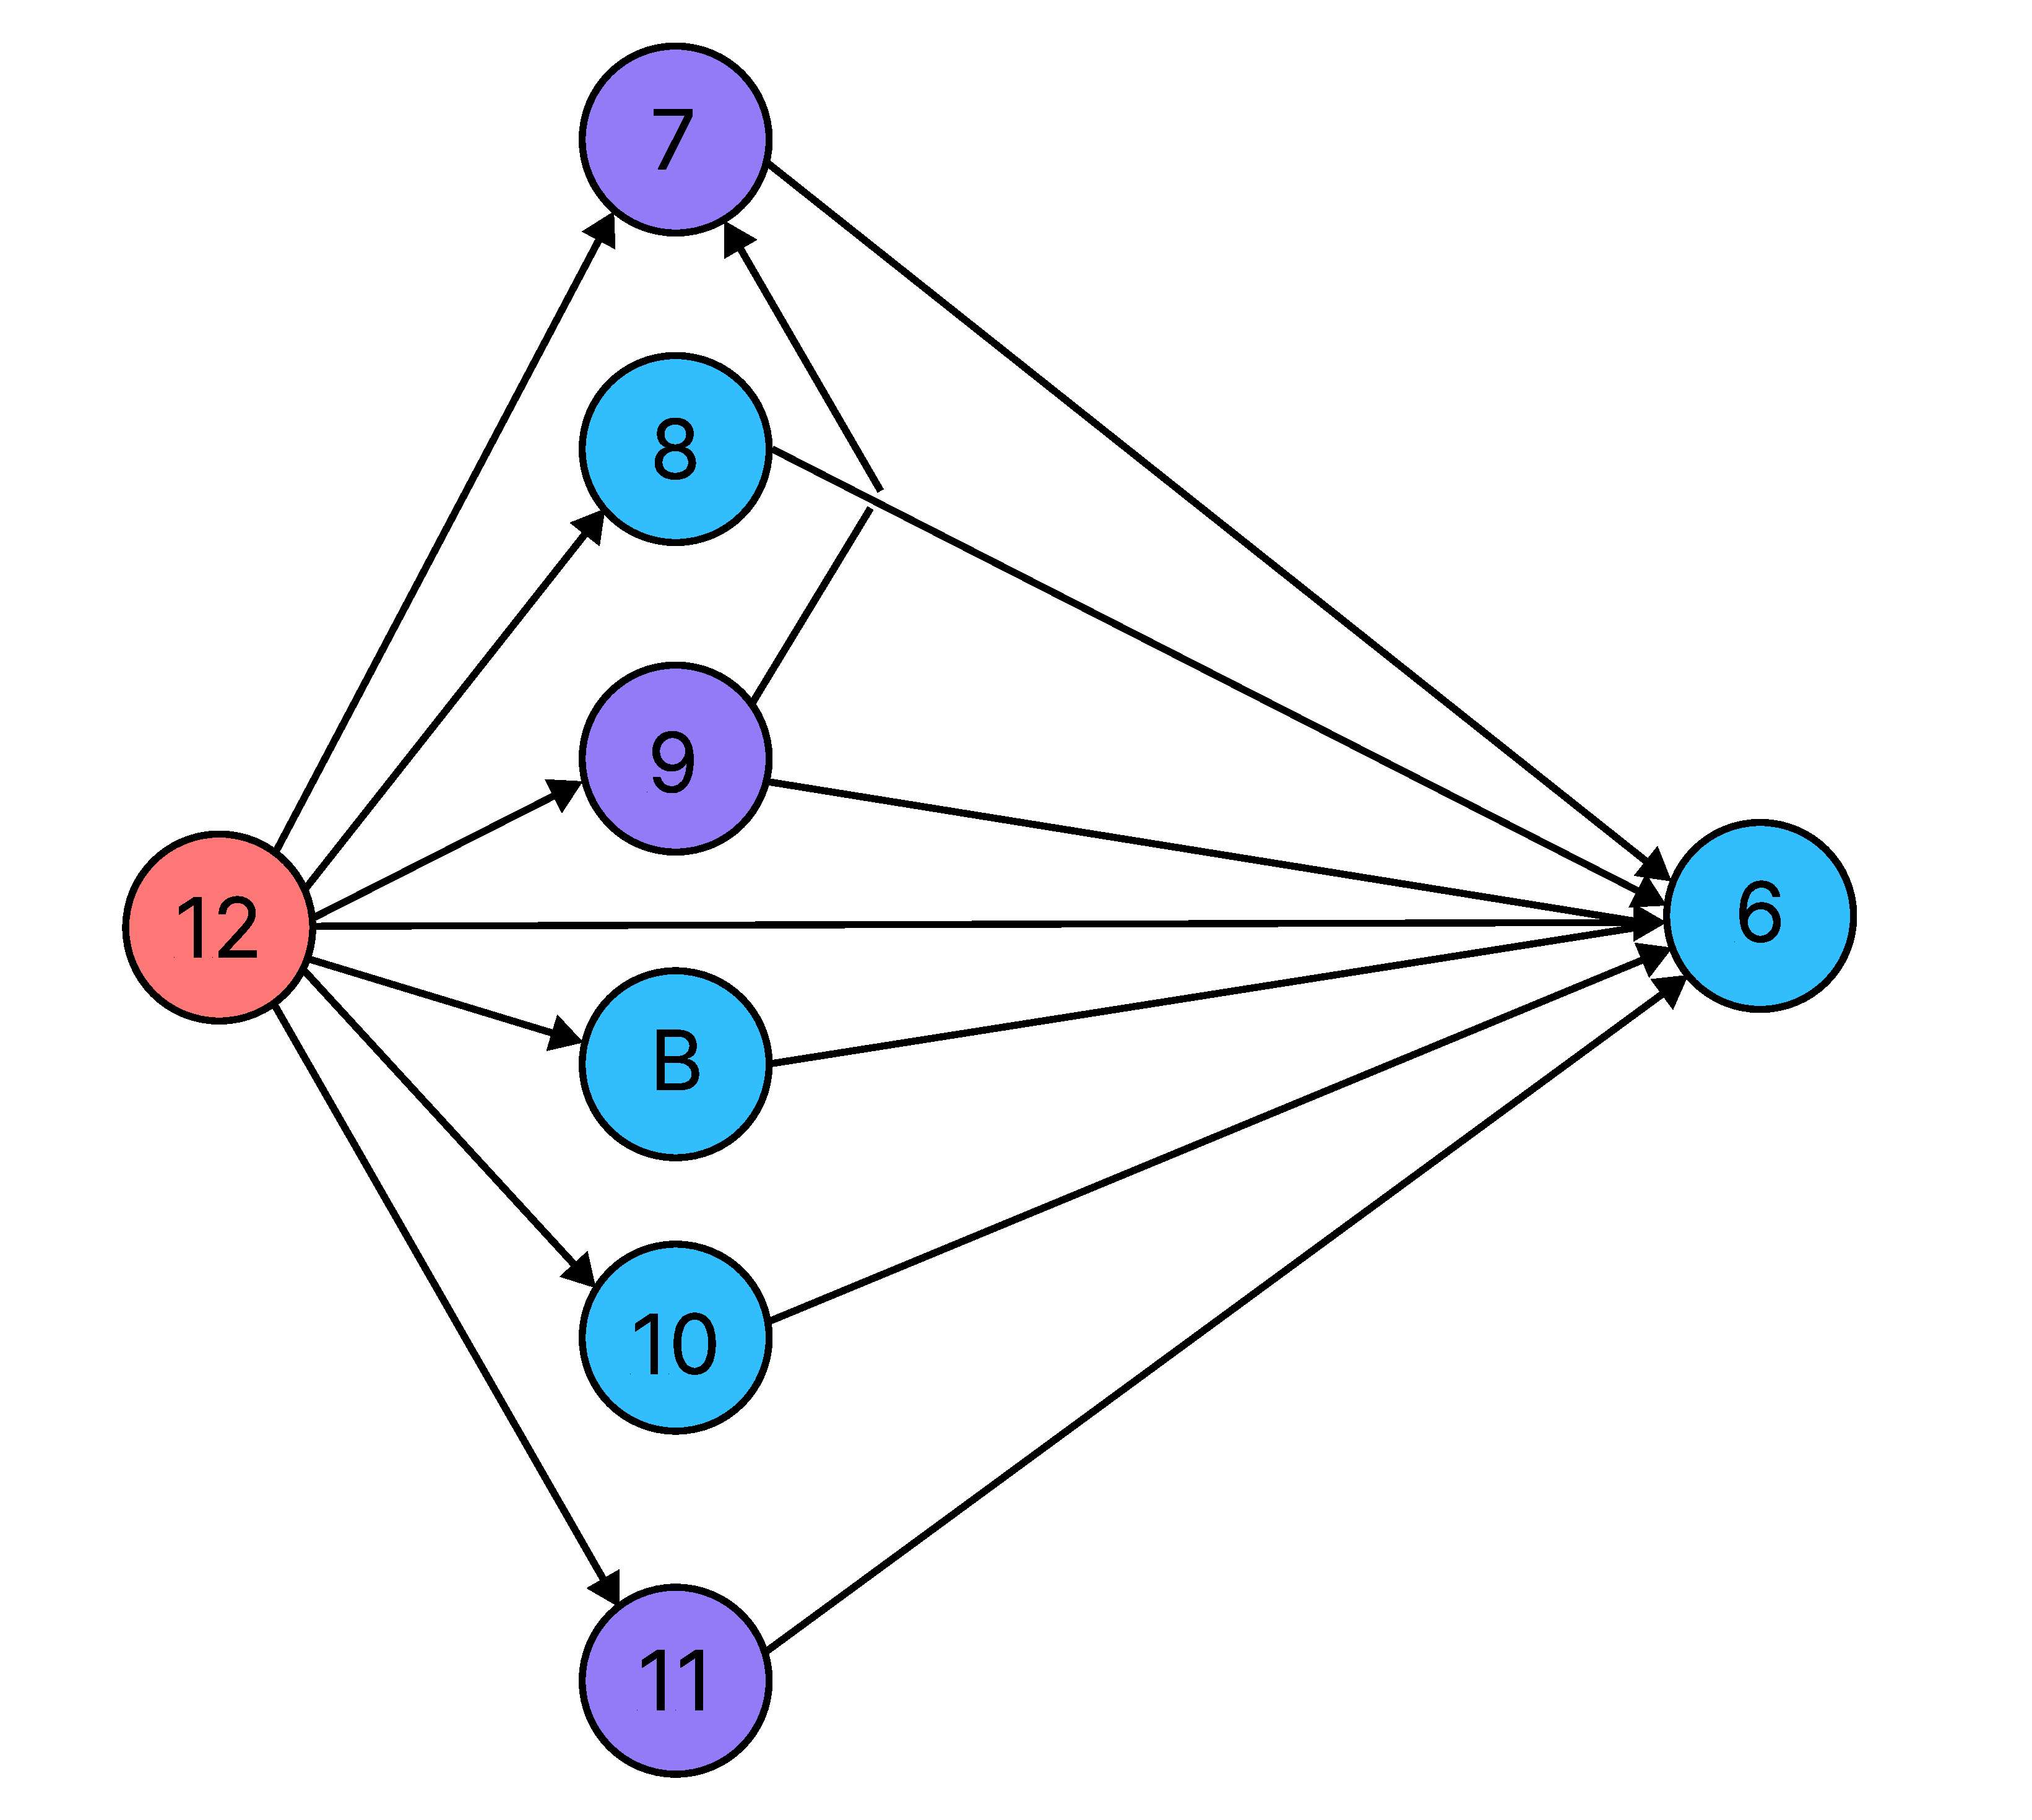
\includegraphics[width=1\textwidth]{sections/images/realated_works_graph}
    ~\caption{Related works graph.}\label{fig:related-works-graph}
\end{figure}
\begin{itemize}
    \item {\Large \textcircled{\normalsize 12}} This manuscript
    \item {\Large \textcircled{\normalsize 6}}
    In \textit{On the link between binomial theorem and discrete convolution}~\cite{on_the_link_between_binomial_theorem_and_discrete_convolution}:
    Let $\mathbf{P}^{m}_{b}(x)$ be a $2m+1$-degree polynomial in $x$ and $b \in \mathbb{R}$
    \[
        \mathbf{P}^{m}_{b}(x) = \sum_{k=0}^{b-1} \sum_{r=0}^{m} \mathbf{A}_{m,r} k^r (x-k)^r
    \]
    where $\mathbf{A}_{m,r}$ are real coefficients.
    In this manuscript, we introduce the polynomial $\mathbf{P}^{m}_{b}(x)$ and study its properties,
    establishing a polynomial identity for odd-powers in terms of this polynomial.
    Based on mentioned polynomial identity for odd-powers,
    we explore the connection between the Binomial theorem and discrete convolution of odd-powers,
    further extending this relation to the multinomial case.
    All findings are verified using Mathematica programs.
    \item {\Large \textcircled{\normalsize 7}}
    In \textit{A study on partial dynamic equation on time scales involving derivatives
    of polynomials}~\cite{study_on_partial_dynamic_eq_on_time_scales_with_poly_derivatives}:
    Extends the main results of {\Large \textcircled{\normalsize 6}} deriving and discussing
    an identity that connects the timescale derivative of odd-powered polynomial
    with partial derivatives of polynomial $\polynomialP{m}{b}{x}$ evaluated in particular points.
    For every $t\in\mathbb{T}_1$ and $(x,b) \in \Lambda^2$
    \[
        \frac{\Delta x^{2m+1}}{\Delta x}(t) =
        \frac{\partial P(m,b,x)}{\Delta x} (m, \sigma(t), t) +
        \frac{\partial P(m,b,x)}{\Delta b} (m, t, t)
    \]
    such that $\sigma(t) > t$ is forward jump operator.
    In addition, we discuss various derivative operators in the context of the partial cases of above equation,
    We show finite difference, classical derivative, $q-$derivative, $q-$power derivative on behalf of it.
    \item {\Large \textcircled{\normalsize 8}}
    In \textit{106.37 An unusual identity for odd-powers}~\cite{unusual_identity_for_odd_powers}:
    Explores and proves the partial case of {\Large \textcircled{\normalsize 6}}
    that is the polynomial identity for odd-powers
    \[
        n^{2m+1} = \sum_{k=1}^{n} \sum_{r=0}^{m} \mathbf{A}_{m,r} k^r (n-k)^r
    \]
    \item {\Large \textcircled{\normalsize 9}}
    In \textit{Another approach to get derivative of odd-power}~\cite{another_approach_to_get_derivative_of_odd_power}:
    Extends the results of {\Large \textcircled{\normalsize 6}} by providing a relation in terms of partial differential equations such that
    ordinary derivative of odd-power $2m+1$ can be reached in terms of partial derivative of the polynomial $\polynomialP{m}{b}{x}$.
    Let be a fixed point $v\in \mathbb{N}$, then ordinary derivative $\frac{d}{dx} g_v (u)$ of the odd-power function $g_v(x) = x^{2v + 1}$
    evaluate in point $u\in\mathbb{R}$ equals to partial derivative $(f_{v})^{'}_{x} (u, u)$ evaluate in point $(u, u)$ plus
    partial derivative $(f_{v})^{'}_{z} (u, u)$ evaluate in point $(u, u)$
    \begin{equation}
        \frac{d}{dx} g_v (u) = (f_{v})^{'}_{x} (u, u) + (f_{v})^{'}_{z} (u, u)
        \label{eq:odd-exponential-identity}
    \end{equation}
    where $f_{y} (x, z) = \sum_{k=1}^{z} \sum_{r=0}^{y} \coeffA{y}{r} k^r (x-k)^r = \polynomialP{y}{z}{x}$.
    \item {\Large \textcircled{\normalsize B}}
    In \textit{A two-sided Faulhaber-like formula involving Bernoulli polynomials}~\cite{barbero2020two}:
    Based on equation~\eqref{eq:rearranging-terms}, the authors give a new identity involving
    Bernoulli polynomials and combinatorial numbers that provides,
    in particular, the Faulhaber-like formula for sums of the form $1^m(n-1)^m + 2^m (n -2)^m + \cdots + (n - 1)^m 1^m$
    for positive integers $m$ and $n$.
    \item {\Large \textcircled{\normalsize 10}}
    In \textit{Polynomial identity involving Binomial Theorem and Faulhaber's formula}~\cite{polynomial_identity_with_binomial_theorem_and_faulhabers_formula}:
    proves that
    for every $n\geq 1, \; n,m\in\mathbb{N}$
    there are coefficients $\mathbf{A}_{m,0}, \mathbf{A}_{m,1}, \ldots, \mathbf{A}_{m,m}$ such that
    the polynomial identity holds
    \[
        n^{2m+1} = \sum_{k=1}^{n} \mathbf{A}_{m,0} k^0 (n-k)^0 + \mathbf{A}_{m,1}(n-k)^1
        + \cdots + \mathbf{A}_{m,m} k^m (n-k)^m
    \]
    which is a direct consequence of the definition of $\polynomialP{m}{b}{x}$ given in {\Large \textcircled{\normalsize 6}},
    reached by utilizing Binomial theorem and Faulhaber's formula.
    \item {\Large \textcircled{\normalsize 11}}
    In \textit{Finding the derivative of polynomials via double limit}~\cite{derivative_of_polynomials_via_double_limit}:
    By applying the results of {\Large \textcircled{\normalsize 6}} provides
    another perspective of ordinary derivatives of polynomials allowing expressing
    them via a double limit, because
    \begin{align*}
        \lim_{h \to 0} \polynomialP{m}{x+h}{x} = x^{2m+1}
    \end{align*}
    \item Three sequences were contributed to the
    OEIS~\cite{oeis_coefficients_u_m_l_k_defined_by_polynomial_identity_1, oeis_coefficients_u_m_l_k_defined_by_polynomial_identity_2, oeis_coefficients_u_m_l_k_defined_by_polynomial_identity_3}
    showing the coefficients of the polynomial $\polynomialP{m}{b}{x}$ having fixed points $m,b$ while $x\in\mathbb{R}$.
    \item OEIS sequences such that row sums give odd-powers~\cite{oeis_numerical_triangle_row_sums_give_cubes, oeis_numerical_triangle_row_sums_give_fifth_powers, oeis_numerical_triangle_row_sums_give_seventh_powers}.
    \item OEIS sequences related to the coefficients $\coeffA{m}{r}$~\cite{oeis_numerators_of_the_coefficient_a_m_r, oeis_denominators_of_the_coefficient_a_m_r}.
\end{itemize}
The node indexes in the related works graph are not random, persisting the same values as
these works have on my personal website
\begin{center}
    \href{https://kolosovpetro.github.io/math/}{\texttt{kolosovpetro.github.io/math}}
\end{center}



    \section{Future research and activities}\label{sec:future-research}
    \begin{itemize}
    \item Differential equation~\eqref{eq:odd-exponential-identity} can also be expressed in terms of backward
    and central differential operators, including derivatives on time-scales so that results of~\cite{study_on_partial_dynamic_eq_on_time_scales_with_poly_derivatives}
    could be generalized further.
    \item Theorem~\eqref{eq:odd-power-theorem} provides an opportunity to express odd-power identity
    in terms of multiplication of certain matrices.
    \item There are Taylor series and Maclaurin series versions in terms of $\polynomialP{m}{b}{x}$.
    \item The summation bounds of definition~\eqref{eq:definition_polynomial_p} can be altered so that
    $k$ runs over $1 \leq k \leq b$, by symmetry.
    \item Prove that $\polynomialP{m}{b}{x}$ is an integer valued polynomial in $(x,b)$.
    \item The definition~\eqref{eq:definition_polynomial_p} is closely related to discrete convolution because
    \begin{equation*}
        \polynomialP{m}{b}{x} = \sum_{r=0}^{m} \coeffA{m}{r} \sum_{k=0}^{b-1} k^r(x-k)^r
    \end{equation*}
    where $\sum_{k=0}^{b-1} k^r(x-k)^r$ is the discrete convolution of $x^r$.
    It is worth to get a closer look into it so that new relations in terms of discrete convolution may be found.
    \item All kinds of derivatives e.g.\ forward, backward and central, including the derivatives on time-scales can be expressed
    as double limit of $\polynomialP{m}{b}{x}$ extending the results of~\cite{derivative_of_polynomials_via_double_limit}.
    \item Introducing the definitions of the coefficients
    $\brackCoefficient{n}{k}{m}$ and $\braceCoefficient{n}{k}{m}$
    \begin{align*}
        \brackCoefficient{n}{k}{m} &= \sum_{r=0}^{m} \coeffA{m}{r} k^r (n-k)^r \\
        \braceCoefficient{n}{r}{m} &= \sum_{k=0}^{n-1} \coeffA{m}{r} k^r (n-k)^r
    \end{align*}
    the novel identities can be reached, for example
    \begin{align*}
        \brackCoefficient{2t+1}{1}{m} &= \brackCoefficient{t+2}{2}{m} \\
        \brackCoefficient{n}{k}{m} &= \brackCoefficient{n}{n-k}{m} \\
        \brackCoefficient{2t-3r}{r}{m} &= \brackCoefficient{t}{2r}{m} = \brackCoefficient{2t-3r}{2t-4r}{m}
    \end{align*}
    so that combinatorial sense of above is also a topic to research.
    \item Contribute new OEIS sequences related to $\brackCoefficient{n}{k}{m}$ and $\braceCoefficient{n}{k}{m}$.
    \item An identity
    \begin{align*}
    (x-2a)
        ^{2m+1} = \sum_{r=0}^{m} \coeffA{m}{r} \sum_{k=a+1}^{x-a} (k-a)^r (x-k-a)^r
    \end{align*}
    allows to provide a novel proof of power rule in terms of derivatives of polynomials.
    \item Following the results of~\url{https://arxiv.org/pdf/1603.02468v15.pdf},
    the equation~\eqref{eq:definition_polynomial_p} approximates the odd-power polynomial $x^{2m+1}$ around given points
    $x_i$ as it may be observed from the following plots
    \begin{figure}[H]
        \centering
        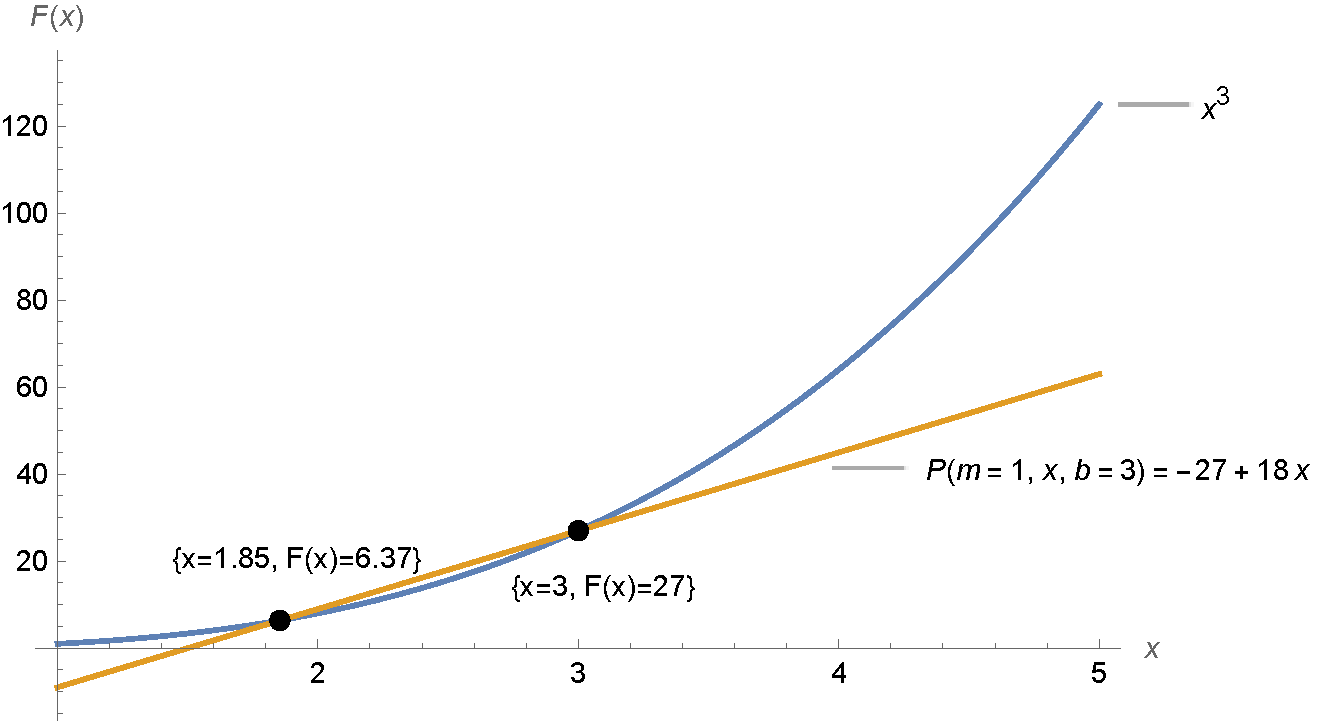
\includegraphics[width=1\textwidth]{sections/images/n^3_approximation_m1_b3}
        ~\caption{Approximation of $x^3$.}\label{fig:approximation-n3}
    \end{figure}
    \begin{figure}[H]
        \centering
        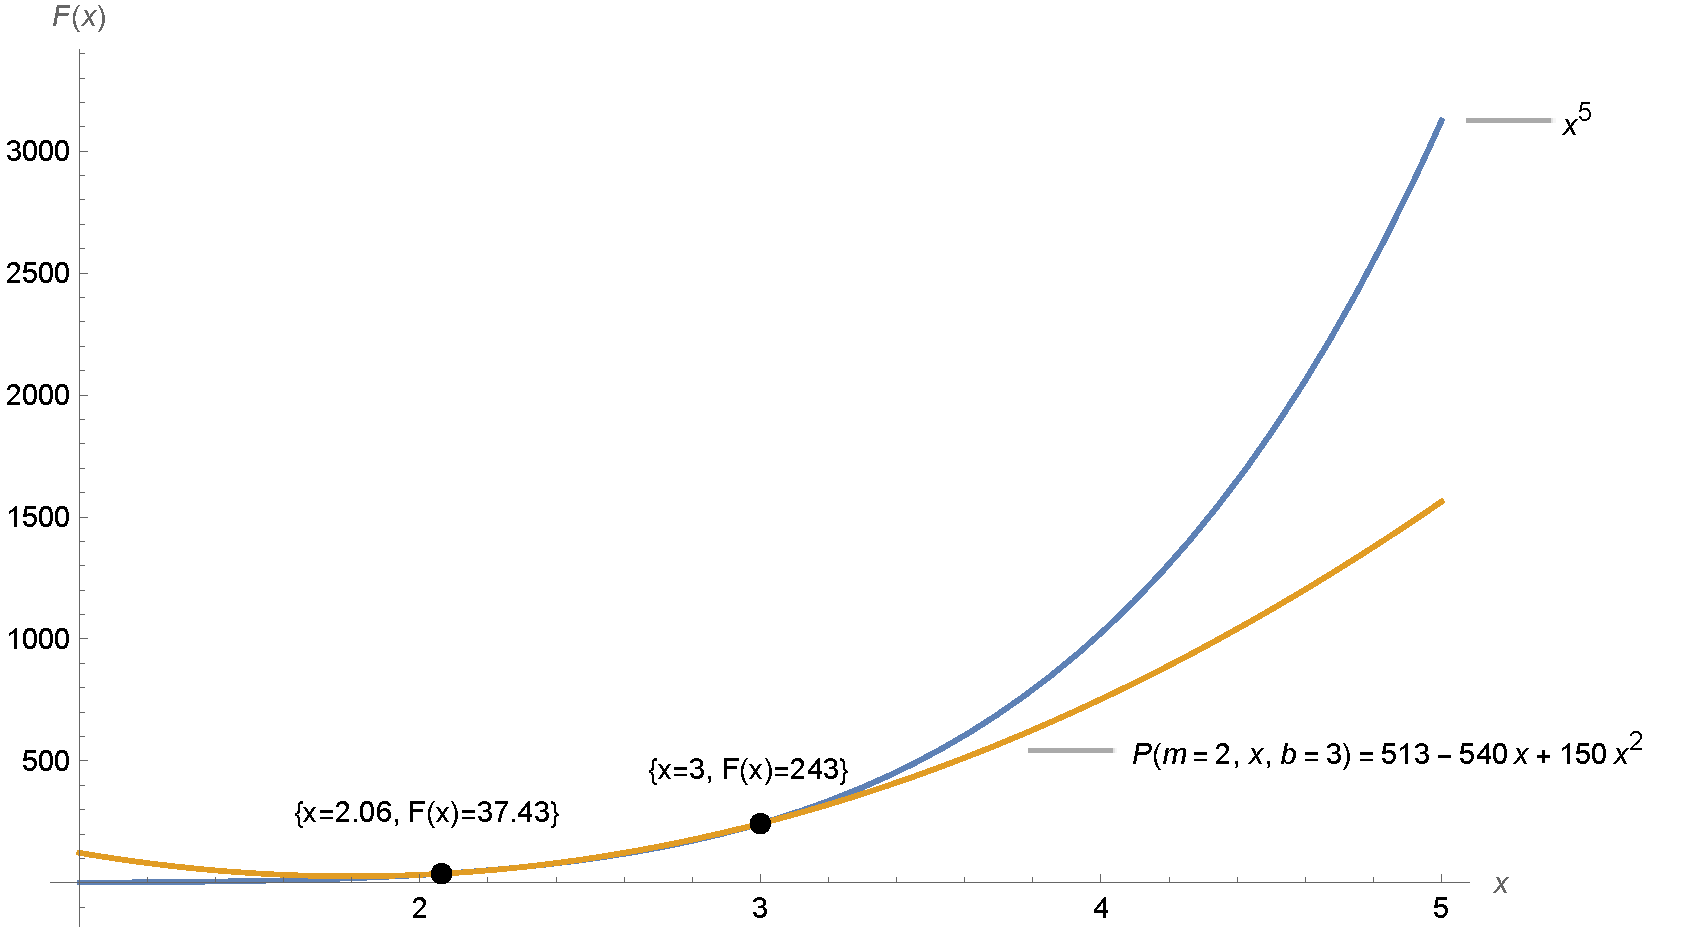
\includegraphics[width=1\textwidth]{sections/images/n^5_approximation_m2_b3}
        ~\caption{Approximation of $x^5$.}\label{fig:approximation-n5}
    \end{figure}
    \item English grammar reviews and improvements are welcome.
    \item Improvements and suggestions to current manuscript under open-source initiatives at
    \url{https://github.com/kolosovpetro/HistoryAndOverviewOfPolynomialP}
\end{itemize}



    \section{Conclusions}\label{sec:conclusions}
    In this manuscript we have successfully provided a comprehensive historical survey
of the milestones and evolution of the polynomial $\polynomialP{m}{b}{x}$
as well as related works such that based onto, for instance various polynomial identities, differential equations etc.
In addition, future research directions are proposed and discussed.


    \bibliographystyle{unsrt}
    \bibliography{surprising-polynomial-identities-classical-interpolation}
    \noindent \textbf{Version:} \texttt{Local-0.1.0}

    \section{Addendum 1: Examples of the polynomial \texorpdfstring{$\polynomialP{m}{b}{x}$}{P[m,b,x]}}
    \label{sec:addendum-1}
    \begin{equation*}
    \begin{split}
        \polynomialP{0}{b}{x}
        &=b \\
        \polynomialP{1}{b}{x}
        &=3 b^2 - 2 b^3 - 3 b x + 3 b^2 x \\
        \polynomialP{2}{b}{x}
        &=10 b^3 - 15 b^4 + 6 b^5- 15 b^2 x + 30 b^3 x - 15 b^4 x + 5 b x^2 - 15 b^2 x^2 + 10 b^3 x^2 \\
        \polynomialP{3}{b}{x}
        &=-7 b^2 + 28 b^3 - 70 b^5 + 70 b^6 - 20 b^7 + 7 b x - 42 b^2 x + 175 b^4 x - 210 b^5 x + 70 b^6 x \\
        &+ 14 b x^2 - 140 b^3 x^2 + 210 b^4 x^2 - 84 b^5 x^2 + 35 b^2 x^3 - 70 b^3 x^3 + 35 b^4 x^3 \\
        \polynomialP{4}{b}{x}
        &= -60 b^2 + 180 b^3 - 294 b^5 + 420 b^7 - 315 b^8 + 70 b^9 + 60 b x - 270 b^2 x + 735 b^4 x - 1470 b^6 x \\
        &+ 1260 b^7 x - 315 b^8 x + 90 b x^2 - 630 b^3 x^2 + 1890 b^5 x^2 - 1890 b^6 x^2 + 540 b^7 x^2 + 210 b^2 x^3 \\
        &- 1050 b^4 x^3 + 1260 b^5 x^3 - 420 b^6 x^3 - 21 b x^4 + 210 b^3 x^4 - 315 b^4 x^4 + 126 b^5 x^4\\
        \polynomialP{5}{b}{x}
        &= -693 b^2 + 2068 b^3 - 330 b^4 - 2640 b^5 + 2772 b^7 - 2310 b^9 + 1386 b^{10} - 252 b^{11} + 693 b x \\
        &- 3102 b^2 x + 660 b^3 x + 6600 b^4 x - 9702 b^6 x + 10395 b^8 x - 6930 b^9 x + 1386 b^{10} x + 1034 b x^2 \\
        &- 330 b^2 x^2 - 5940 b^3 x^2 + 12936 b^5 x^2 - 18480 b^7 x^2 + 13860 b^8 x^2 - 3080 b^9 x^2 + 2310 b^2 x^3 \\
        &- 8085 b^4 x^3 + 16170 b^6 x^3 - 13860 b^7 x^3 + 3465 b^8 x^3 - 330 b x^4 + 2310 b^3 x^4 - 6930 b^5 x^4 \\
        &+ 6930 b^6 x^4 - 1980 b^7 x^4 - 231 b^2 x^5 + 1155 b^4 x^5 - 1386 b^5 x^5 + 462 b^6 x^5 \\
        \polynomialP{6}{b}{x}
        &= -10920 b^2 + 33306 b^3 - 9009 b^4 - 36036 b^5 + 37752 b^7 - 22022 b^9 + 12012 b^{11} - 6006 b^{12} + 924 b^{13} \\
        &+ 10920 b x - 49959 b^2 x + 18018 b^3 x + 90090 b^4 x - 132132 b^6 x + 99099 b^8 x - 66066 b^{10} x + 36036 b^{11} x \\
        &- 6006 b^{12} x + 16653 b x^2 - 9009 b^2 x^2 - 84084 b^3 x^2 + 180180 b^5 x^2 - 180180 b^7 x^2 + 150150 b^9 x^2 \\
        &- 90090 b^{10} x^2 + 16380 b^{11} x^2 + 36036 b^2 x^3 - 120120 b^4 x^3 + 168168 b^6 x^3 - 180180 b^8 x^3 \\
        &+ 120120 b^9 x^3 - 24024 b^{10} x^3 - 6006 b x^4 + 40040 b^3 x^4 - 84084 b^5 x^4 + 120120 b^7 x^4 - 90090 b^8 x^4 \\
        &+ 20020 b^9 x^4 - 6006 b^2 x^5 + 21021 b^4 x^5 - 42042 b^6 x^5 + 36036 b^7 x^5 - 9009 b^8 x^5 + 286 b x^6 \\
        &- 2002 b^3 x^6 + 6006 b^5 x^6 - 6006 b^6 x^6 + 1716 b^7 x^6
    \end{split}
\end{equation*}



    \section{Addendum 2: Derivation of the coefficients \texorpdfstring{$\coeffA{m}{r}$}{A[m,r]}}
    \label{sec:addendum-2}
    Consider the definition~\eqref{eq:definition_coefficient_a} of the coefficients $\coeffA{m}{r}$, it can be written as
\begin{equation*}
    \coeffA{m}{r} =
    \begin{cases}
    (2r+1)
        \binom{2r}{r}, & \text{if } r=m; \\
        \sum_{d \geq 2r+1}^{m} \coeffA{m}{d} \underbrace{(2r+1) \binom{2r}{r} \binom{d}{2r+1} \frac{(-1)^{d-1}}{d-r} \bernoulli{2d-2r}}_{T(d,r)}, & \text{if } 0 \leq r<m; \\
        0, & \text{if } r<0 \text{ or } r>m,
    \end{cases}
\end{equation*}
Therefore, let be a definition of the real coefficient $T(d,r)$
\begin{definition}
    Real coefficient $T(d,r)$
    \begin{equation*}
        T(d,r) = (2r+1) \binom{2r}{r} \binom{d}{2r+1} \frac{(-1)^{d-1}}{d-r} \bernoulli{2d-2r}
    \end{equation*}
\end{definition}
\begin{example}
    Let be $m=2$ so first we get $\coeffA{2}{2}$
    \begin{equation*}
        \coeffA{2}{2} = 5\binom{4}{2}=30
    \end{equation*}
    Then $\coeffA{2}{1} = 0$ because $\coeffA{m}{d}$ is zero in the range $m/2 \leq d < m$ means that zero for $d$
    in $1 \leq d < 2$.
    Finally, the coefficient $\coeffA{2}{0}$ is
    \begin{equation*}
        \begin{split}
            \coeffA{2}{0}
            = \sum_{d \geq 1}^{2} \coeffA{2}{d} \cdot T(d, 0)
            &= \coeffA{2}{1} \cdot T(1, 0) + \coeffA{2}{2} \cdot T(2, 0) \\
            &= 30 \cdot \frac{1}{30} = 1
        \end{split}
    \end{equation*}
\end{example}
\begin{example}
    Let be $m=3$ so that first we get $\coeffA{3}{3}$
    \begin{equation*}
        \coeffA{3}{3} = 7 \binom{6}{3}= 140
    \end{equation*}
    Then $\coeffA{3}{2} = 0$ because $\coeffA{m}{d}$ is zero in the range $m/2 \leq d < m$ means that zero for $d$
    in $2 \leq d < 3$.
    The $\coeffA{3}{1}$ coefficient is non-zero and calculated as
    \begin{equation*}
        \begin{split}
            \coeffA{3}{1} = \sum_{d \geq 3}^{3} \coeffA{3}{d} \cdot T(d,1) = \coeffA{3}{3} \cdot T(3,1)
            = 140 \cdot \left( -\frac{1}{10} \right) = -14
        \end{split}
    \end{equation*}
    Finally, the coefficient $\coeffA{3}{0}$ is
    \begin{equation*}
        \begin{split}
            \coeffA{3}{0}= \sum_{d \geq 1}^{3} \coeffA{3}{d} \cdot T(d,0)
            &= \coeffA{3}{1} \cdot T(1,0) + \coeffA{3}{2} \cdot T(2,0) + \coeffA{3}{3} \cdot T(3,0) \\
            &= -14 \cdot \frac{1}{6} + 140 \cdot \frac{1}{42} = 1
        \end{split}
    \end{equation*}
\end{example}
\begin{example}
    Let be $m=4$ so that first we get $\coeffA{4}{4}$
    \begin{equation*}
        \coeffA{4}{4} = 9 \binom{8}{4}= 630
    \end{equation*}
    Then $\coeffA{4}{3} = 0$ and $\coeffA{4}{2} = 0$
    because $\coeffA{m}{d}$ is zero in the range $m/2 \leq d < m$ means that zero for $d$ in $2 \leq d < 4$.
    The value of the coefficient $\coeffA{4}{1}$ is non-zero and calculated as
    \begin{equation*}
        \begin{split}
            \coeffA{4}{1}
            = \sum_{d \geq 3}^{4} \coeffA{4}{d} \cdot T(d,1)
            = \coeffA{4}{3} \cdot T(3,1) + \coeffA{4}{4} \cdot T(4,1)
            = 630 \cdot \left( -\frac{4}{21} \right)
            = -120
        \end{split}
    \end{equation*}
    Finally, the coefficient $\coeffA{4}{0}$ is
    \begin{equation*}
        \begin{split}
            \coeffA{4}{0}
            = \sum_{d \geq 1}^{4} \coeffA{4}{d} \cdot T(d, 0)
            = \coeffA{4}{1} \cdot T(1, 0) + \coeffA{4}{4} \cdot T(4, 0)
            = -120 \cdot \frac{1}{6} + 630 \cdot \frac{1}{30} = 1
        \end{split}
    \end{equation*}
\end{example}
\begin{example}
    Let be $m=5$ so that first we get $\coeffA{5}{5}$
    \begin{equation*}
        \coeffA{5}{5} = 11 \binom{10}{5}= 2772
    \end{equation*}
    Then $\coeffA{5}{4} = 0$ and $\coeffA{5}{3} = 0$
    because $\coeffA{m}{d}$ is zero in the range $m/2 \leq d < m$ means that zero for $d$ in $3 \leq d < 5$.
    The value of the coefficient $\coeffA{5}{2}$ is non-zero and calculated as
    \begin{equation*}
        \begin{split}
            \coeffA{5}{2}
            = \sum_{d \geq 5}^{5} \coeffA{5}{d} \cdot T(d,2) = \coeffA{5}{5} \cdot T(5,2) = 2772 \cdot \frac{5}{21} = 660
        \end{split}
    \end{equation*}
    The value of the coefficient $\coeffA{5}{1}$ is non-zero and calculated as
    \begin{equation*}
        \begin{split}
            \coeffA{5}{1}
            &= \sum_{d \geq 3}^{5} \coeffA{5}{d} \cdot T(d,1)
            = \coeffA{5}{3} \cdot T(3,1) + \coeffA{5}{4} \cdot T(4,1) + \coeffA{5}{5} \cdot T(5,1) \\
            &= 2772 \cdot \left( - \frac{1}{2} \right) = -1386
        \end{split}
    \end{equation*}
    Finally, the coefficient $\coeffA{5}{0}$ is
    \begin{equation*}
        \begin{split}
            \coeffA{5}{0}
            &= \sum_{d \geq 1}^{5} \coeffA{5}{d} \cdot T(d, 0)
            = \coeffA{5}{1} \cdot T(1, 0) + \coeffA{5}{2} \cdot T(2, 0) + \coeffA{5}{5} \cdot T(5, 0) \\
            &= -1386 \cdot \frac{1}{6} + 660 \cdot \frac{1}{30} + 2772 \cdot \frac{5}{66} = 1
        \end{split}
    \end{equation*}
\end{example}



    \section{Addendum 3: Odd power identities}
    \label{sec:addendum-3}
    \begin{align*}
    n^3 &= \sum_{k=1}^{n} 6k(n-k) + 1 \\
    n^5 &= \sum_{k=1}^{n} 30k^2(n-k)^2 + 1 \\
    n^7 &= \sum_{k=1}^{n} 140 k^3 (n-k)^3 - 14k(n-k) + 1 \\
    n^9 &= \sum_{k=1}^{n} 630 k^4(n-k)^4 - 120k(n-k) + 1 \\
    n^{11} &= \sum_{k=1}^{n} 2772 k^5(n-k)^5 + 660 k^2(n-k)^2 - 1386k(n-k) + 1 \\
    n^{13} &= \sum_{k=1}^{n} 51480 k^7(n-k)^7 - 60060 k^3(n-k)^3 + 491400k^2(n-k)^{2} - 450054k(n-k) + 1 \\
\end{align*}


\end{document}
